\subsection{Data Generators} \label{sec:data-generators}

Creating new data from existing data is known as generative modeling. This technique has numerous applications across various media types, including images, text, and video. However, each media type possesses unique characteristics, so generating them requires distinct approaches and techniques. Sound, for instance, presents a different set of challenges than other media types, and hence its generation necessitates diverse techniques.

This section aims to survey some of the state-of-the-art generators for media types that are not sound-based, primarily focusing on image generators. By doing so, one hopes to comprehensively understand the different approaches and techniques employed for generating various media types.

The discussion delves into the main ideas behind these generators, their strengths and limitations, and how they can be related to or inspired by sound generation. Through this exploration, this section highlights the diversity of methods used for generative modeling and how they can be adapted to different contexts.

\begin{table}[ht]
\centering
\caption{Comparison of Data Generators}
\begin{tabularx}{\textwidth}{|X|X|X|X|}
\hline
\textbf{Generator Name} & \textbf{Main Idea}                                                                                                                    & \textbf{Strengths}                                                                                                                                 & \textbf{Limitations}                                                                                                          \\ \hline
PixelCNN~\cite{oord_conditional_2016}                & Uses autoregressive connections to model images pixel by pixel.                                                                       & Fast and parallelizable training, high resolution and diversity, interpretable latent space.                                                       & Slow and sequential sampling, limited global coherence, difficulty in conditioning on high-level features.                    \\ \hline
DALL-E~\cite{ramesh_zero-shot_2021}                  & A transformer language model that creates images from text descriptions, using a dataset of text–image pairs.                         & Can generate novel and creative images, combine concepts in plausible ways, render text and apply transformations.                                 & Requires large amounts of data and compute, may produce harmful or biased outputs, not publicly accessible.                   \\ \hline
Stable Diffusion~\cite{rombach_high-resolution_2021}        & A latent diffusion model that creates images from text descriptions, using a dataset of text–image pairs and a pretrained CLIP model. & Can generate realistic and detailed images, is lighter than previous state of the art models.                                                      & Requires fine-tuning for specific domains, may produce artifacts or inconsistencies, sensitive to text prompts.               \\ \hline
GLIDE~\cite{nichol_glide_2021}                   & Guided diffusion-based approach for text-conditioned image generation.                                                                & High-fidelity image synthesis, classifier-free guidance preferred for photorealism and caption similarity, text-driven image editing capabilities. & Difficulty generating images for complex or unusual text prompts, slow generation speed.                                      \\ \hline
DALL-E 2~\cite{ramesh_hierarchical_2022}                & An improved version of DALL-E that generates more realistic and accurate images using a diffusion model.                              & Has better results than DALL-E and is faster.                                                                                                      & Still requires large amounts of data and compute, may still produce harmful or biased outputs, still not publicly accessible. \\ \hline
\end{tabularx}
\label{tab:data-generators}
\end{table}

\subsubsection{PixelCNN Decoders} \label{sec:pixelcnn}

Van den Oord et al. introduced \textit{PixelCNNs} as discussed in \cite{oord_conditional_2016, van_den_oord_pixel_2016}. PixelCNNs model high-dimensional discrete data, like images.

They employ the \ac{AE} architecture as described in Section \ref{sec:darn}, where pixels are generated sequently while conditioning on prior pixels.

The goal is to estimate a distribution over images that can be used to compute the likelihood of images and thus generate new ones. The network scans the image one row at a time and one pixel at a time within each row, using masked convolutions (see Section~\ref{sec:masked-conv}). For each pixel, it predicts the conditional distribution over the possible pixel values given the scanned context.

Each image $x$ is assigned a probability $p(x)$. To do this, if one considers each pixel sequentially, row by row, such that $x_k$ is the pixel number $k$, the final probability is as follows.

\begin{equation}
    p(x) = \prod_{i=1}^{h \times w} p(x_i | x_1, \dots, x_{i-1})
\end{equation}

Where $h$ is the height of the image and $w$ is the width.

For multiple colors, one can condition the colors on one another. For instance, instead of having $x_1$, $x_2$, \dots, there would be $x_1^R$, $x_1^G$, $x_1^B$, $x_2^R$, and so forth.
\begin{tikzpicture}[font=\small]
	\begin{pgfonlayer}{nodelayer}
		\node [style=input] (0) at (11, -8) {};
		\node [style=input] (1) at (14, -8) {};
		\node [style=input] (2) at (17, -8) {};
		\node [style=input] (3) at (8, -8) {};
		\node [style=input] (4) at (5, -8) {};
		\node [style=neuron] (6) at (14, -11) {};
		\node [style=neuron] (7) at (11, -11) {};
		\node [style=neuron] (8) at (8, -11) {};
		\node [style=neuron] (13) at (14, -21) {};
		\node [style=neuron] (14) at (11, -21) {};
		\node [style=neuron] (15) at (8, -21) {};
		\node [style=output] (17) at (14, -24) {};
		\node [style=output] (18) at (11, -24) {};
		\node [style=output] (19) at (8, -24) {};
		\node [style=output] (20) at (5, -24) {};
		\node [style=output] (21) at (17, -24) {};
		\node [style=none] (41) at (11.5, -14.25) {};
		\node [style=none] (42) at (11.5, -17.75) {};
		\node [style=none] (43) at (11, -14) {};
		\node [style=none] (44) at (10.5, -14.25) {};
		\node [style=none] (45) at (11, -18) {};
		\node [style=none] (46) at (10.5, -17.75) {};
		\node [style=blue square] (47) at (11, -16) {};
		\node [style=blue square] (48) at (13, -16) {};
		\node [style=blue square] (49) at (15, -16) {};
		\node [style=blue square] (50) at (9, -16) {};
		\node [style=blue square] (51) at (7, -16) {};
		\node [style=transformer rect] (53) at (0, -16) {Transformer Decoder};
		\node [style=main rect] (58) at (-9, -16) {``A dog wearing pants''};
	\end{pgfonlayer}
	\begin{pgfonlayer}{edgelayer}
		\draw [style=input->neuron] (2) to (6);
		\draw [style=input->neuron] (2) to (7);
		\draw [style=input->neuron] (2) to (8);
		\draw [style=input->neuron] (0) to (6);
		\draw [style=input->neuron] (3) to (7);
		\draw [style=input->neuron] (4) to (8);
		\draw [style=input->neuron] (1) to (6);
		\draw [style=input->neuron] (1) to (7);
		\draw [style=input->neuron] (1) to (8);
		\draw [style=input->neuron] (0) to (7);
		\draw [style=input->neuron] (3) to (8);
		\draw [style=input->neuron] (0) to (8);
		\draw [style=input->neuron] (3) to (6);
		\draw [style=input->neuron] (4) to (7);
		\draw [style=input->neuron] (4) to (6);
		\draw [style=neuron->output] (13) to (17);
		\draw [style=neuron->output] (13) to (18);
		\draw [style=neuron->output] (13) to (19);
		\draw [style=neuron->output] (13) to (20);
		\draw [style=neuron->output] (14) to (17);
		\draw [style=neuron->output] (14) to (18);
		\draw [style=neuron->output] (14) to (19);
		\draw [style=neuron->output] (14) to (20);
		\draw [style=neuron->output] (15) to (21);
		\draw [style=neuron->output] (15) to (17);
		\draw [style=neuron->output] (15) to (18);
		\draw [style=neuron->output] (15) to (19);
		\draw [style=neuron->output] (15) to (20);
		\draw [style=neuron->neuron] (6) to (41.center);
		\draw [style=neuron->neuron] (42.center) to (13);
		\draw [style=neuron->neuron] (7) to (43.center);
		\draw [style=neuron->neuron] (8) to (44.center);
		\draw [style=neuron->neuron] (45.center) to (14);
		\draw [style=neuron->neuron] (46.center) to (15);
		\draw [style=input->neuron] (58) to (53);
		\draw [style=neuron->output] (14) to (21);
		\draw [style=neuron->output] (13) to (21);
		\draw [style=->input] (53) to (51);
	\end{pgfonlayer}
\end{tikzpicture}

\subsubsection{Stable Diffusion} \label{sec:stable-diffusion}

Stable Diffusion \cite{rombach_high-resolution_2021} rose from the idea of democratization high-resolution images. According to the original paper, high-end models demand hundreds of thousands of dollars to be trained solely due to their complexities. These models generally operate directly on the pixel space. The training and evaluation of such models necessitate significant computational resources, which are typically only available to the largest companies, thereby contributing to significant carbon footprints.

They apply the diffusion process (see Section \ref{sec:diffusion}) in pre-trained \acp{AE}' (Section \ref{sec:autoencoders}) latent space to optimize the diffusion model practice instead of directly on the pixel space.

For this stable diffusion model, training is separated into two phases: the training of the \ac{AE} and the training of the diffusion model.

One needs the text and Gaussian noise to infer new images given text. The text is embedded using a transformer (see Section \ref{sec:transformers}). In order to increase the relation between the text and the generated image, the text embeddings for an empty string are also generated.

The model takes the initial noise, text and audio embeddings, and timestamp as inputs. Through inverse diffusion process, it generates two new images: one conditioned on the real embeddings, and another with no embeddings (empty string embedding). The image generated by the real embeddings is a synthesis conditioned on the given text and audio input. On the other hand, generating an image without any embeddings produces a random image unconditioned by the provided text or audio. At each step of diffusion process, the model compares the two images to evaluate their differences. By increasing this difference, the final output image becomes conditioned on the initial textual input to a greater extent.

The U-Nets in the diffusion process use cross-attention mechanisms for their respective embeddings (refer to Section \ref{sec:u-net}). Cross-attention extends attention mechanisms used in neural networks. Self-attention captures relationships within a single sequence or embedding, while cross-attention captures dependencies between different sequences or embeddings.

In this study, the U-Nets use cross-attention to allow information exchange and interaction between audio features and other modalities, including text embeddings or image representations. Using cross-attention in the diffusion process improves the model's ability to consider local and global contextual cues from multiple sources during audio synthesis.

Using cross-attention allows different parts of the network to attend to each other's information, enabling better integration and coherence across various modalities involved in generating soundscapes from textual input. This comprehensive modeling improves the overall performance.

After the diffusion process is completed, the decoder takes the generated image embeddings and generates a new image.

This process can be seen in Figure \ref{fig:stable-diffusion}.

\begin{figure}[ht]
    \centering
    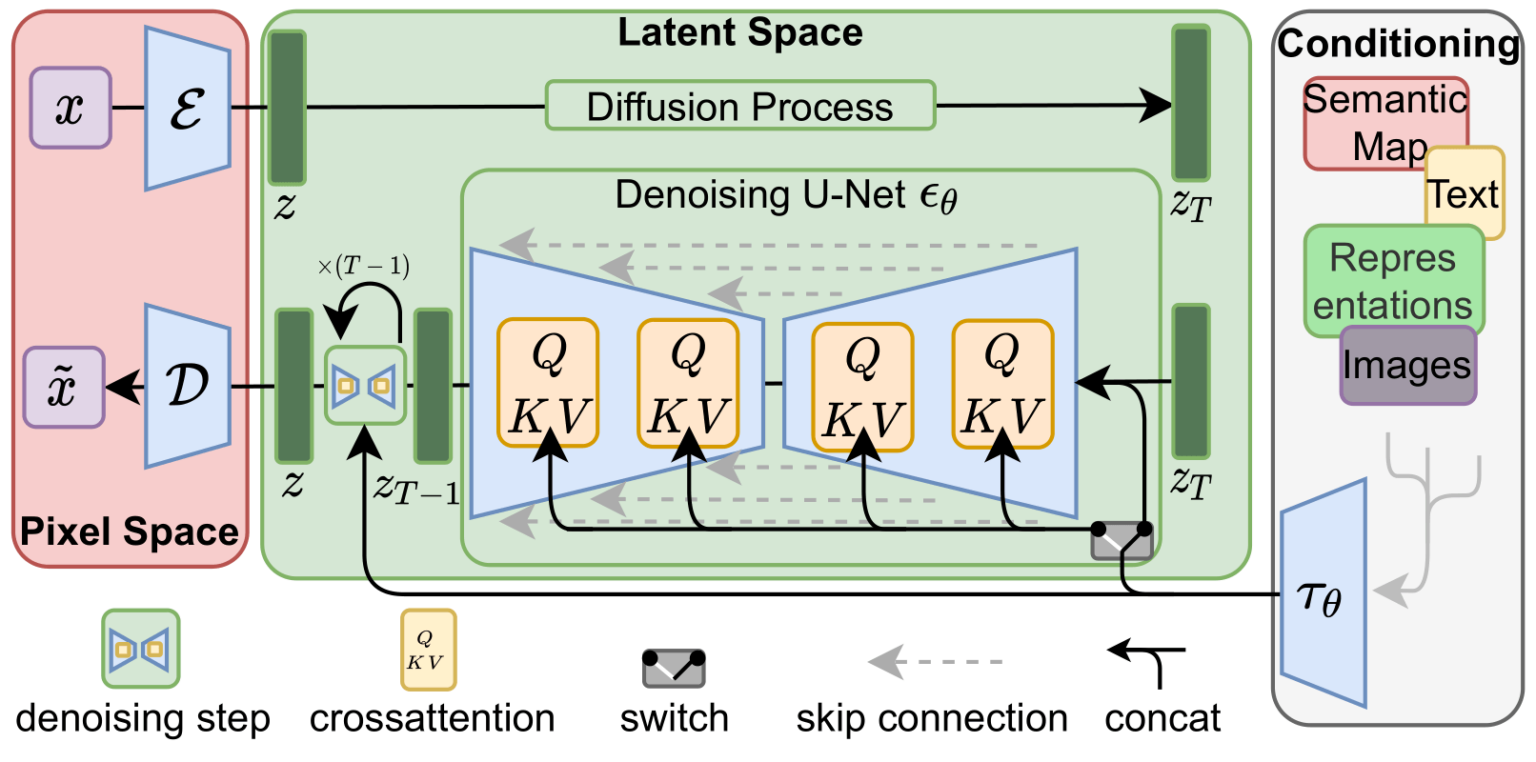
\includegraphics[width=\textwidth]{figures/2-sota/stable-diffusion.png}
    \caption[Stable diffusion architecture]{\textbf{Stable diffusion architecture} --- The Figure was taken from the original paper. On the top left, the original image $x$ is encoded with the \ac{AE}, and the diffusion process happens with the encodings. The text (or another data kind) is encoded with a transformer $\tau_{\theta}$, and these encodings are applied with attention to the denoising U-Nets. This denoising U-Net is applied $T$ times before the decoder transforms the encodings into an actual image in the pixel space again.}
    \label{fig:stable-diffusion}
\end{figure}
\subsubsection{GLIDE} \label{sec:glide}

The \acf{GLIDE} model is a state-of-the-art approach for generating high-fidelity synthetic images from free-form natural-language text prompts. The model is based on a guided diffusion-based approach, which is the first attempt by OpenAI at text-conditioned image generation using guided diffusion. The approach involves two types of guidance strategies during model training: classifier-free guidance~\cite{ho_classifier-free_2022}, which relies solely on the model's knowledge, and \ac{CLIP} guidance which uses a pre-trained \ac{CLIP} model~\cite{radford_learning_2021} to provide guidance based on caption matching.

The experimental results of the \ac{GLIDE} paper demonstrate several benefits of the proposed approach. Human evaluators preferred images generated with classifier-free guidance over \ac{CLIP} guidance regarding photorealism and caption similarity. Samples from the 3.5 billion parameter \ac{GLIDE} model were also found to outperform DALL-E (see Section~\ref{fig:dall-e}) samples according to human evaluations. Additionally, the model can perform text-driven image editing tasks beyond zero-shot image generation from text prompts. Text-driven image editing refers to editing existing images according to text prompts, such as changing attributes or objects within an image as directed by the text.

Despite its success, the \ac{GLIDE} model has some limitations. It fails to generate images for some complex or unusual text prompts. Moreover, the model's generation speed is slow, taking several seconds to generate one image on a flagship \ac{GPU}. Possible solutions to address these limitations include improving the model architecture, optimization techniques, and combining \ac{GLIDE} with faster \ac{GAN}-based methods.

\Acf{CLIP} refers to a model trained to determine if an image and text caption match. It consists of a transformer-based text encoder (see Section \ref{sec:transformers}) and a convolutional neural network-based image encoder (see Section \ref{sec:CNN}). The text encoder produces an embedding of the text, and the image encoder produces an embedding of the image. These embeddings are then compared, and during training, the model learns to produce similar embeddings for matching image-text pairs and dissimilar embeddings for mismatching pairs. This contrastive learning approach allowed CLIP to learn cross-modal understanding between text and images in an unsupervised manner. The pre-trained CLIP model can provide additional guidance to other text-to-image models, such as \ac{GLIDE}, by scoring how well-generated images match given text prompts.
\subsubsection{DALL-E 2} \label{sec:dall-e-2}

\textit{DALL-E 2} is a model proposed by researchers at OpenAI capable of generating images given a textual prompt~\cite{ramesh_hierarchical_2022}. This model can also modify given images, but this use case is not so interesting for the work present in this thesis.

The model consists of two blocks: the prior and the decoder. The prior converts captions into a lower-level representation, while the decoder turns this representation into an actual image.

They use \ac{CLIP} \cite{radford_learning_2021} and GLIDE (see Section~\ref{sec:glide}). For DALLE-2, the text is initially embedded using \ac{CLIP} embeddings. Then, the role of the prior is to translate these embeddings into embeddings related to an image and not the text itself. In other words, create an image representation with textual embeddings. For this, the researchers tried an \ac{AR} and a diffusion model. The diffusion one yielded better results (see Sections~\ref{sec:darn} and~\ref{sec:diffusion}). The decoder then takes the generated image representation and generates the image. The whole process can be seen in Figure \ref{fig:dall-e-2}.

\begin{figure}[ht]
    \centering
    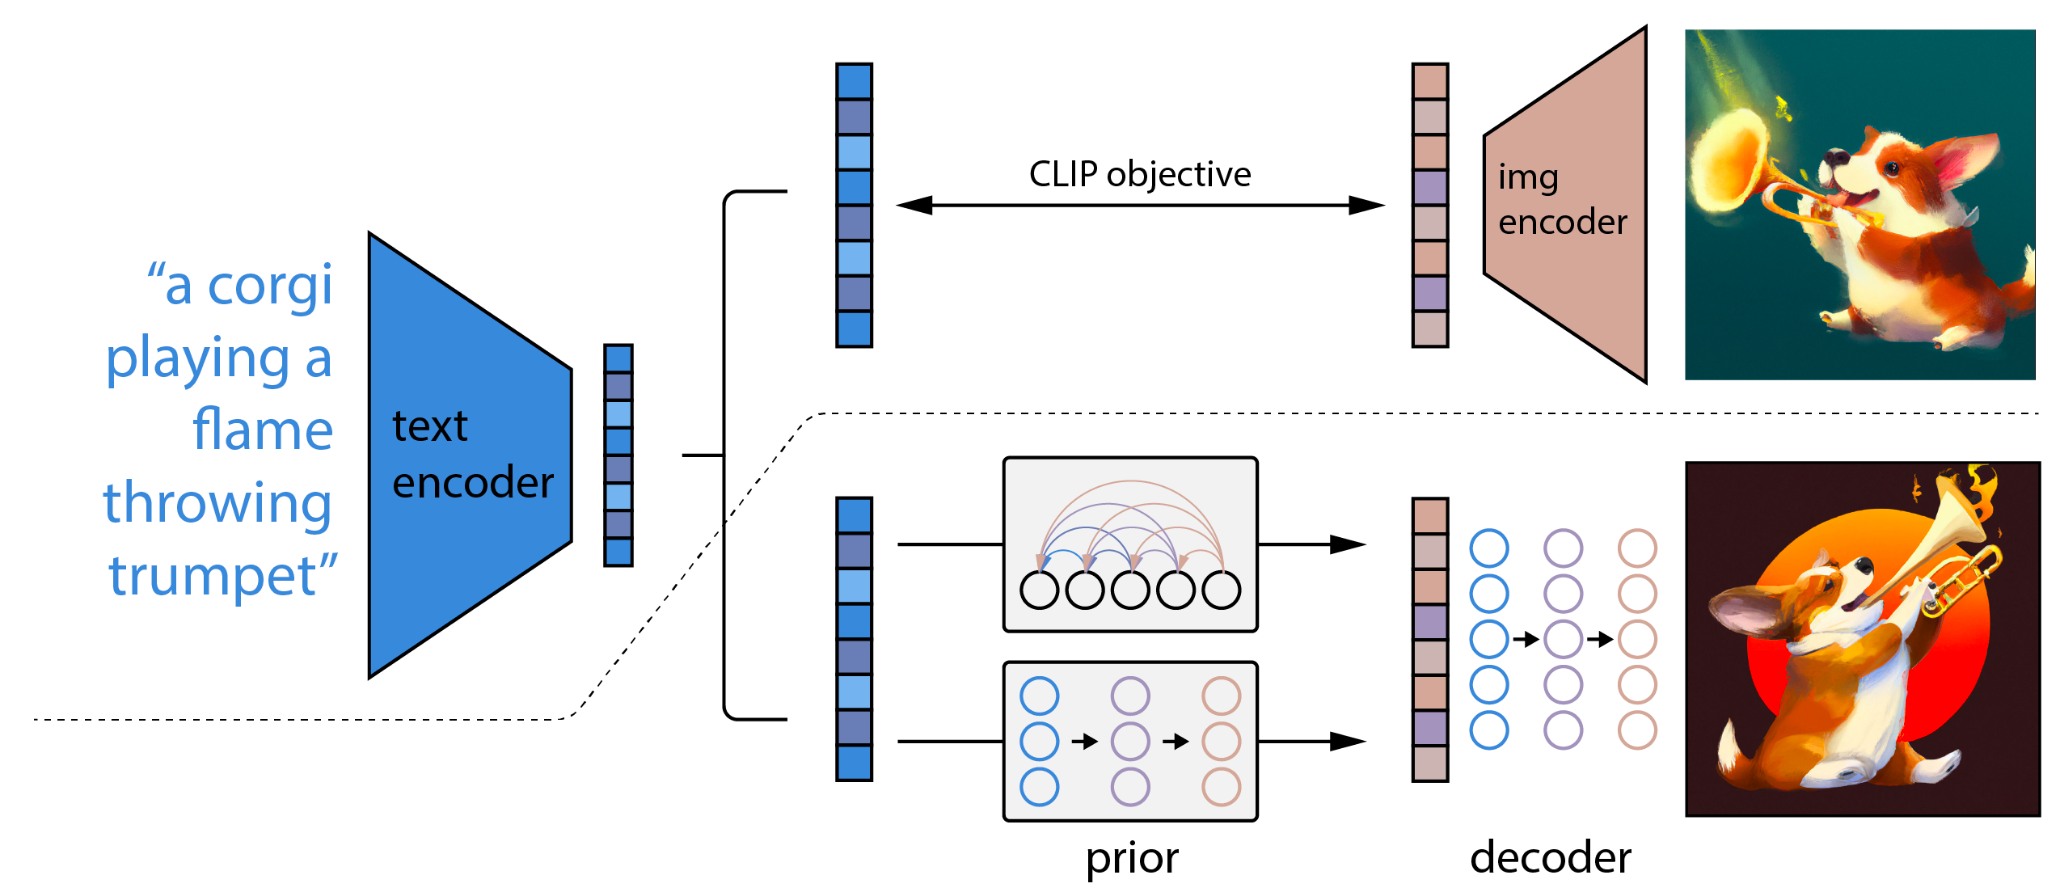
\includegraphics[width=\textwidth]{figures/2-sota/dall-e-2.png}
    \caption[DALL-E 2 architecture]{\textbf{DALL-E 2 architecture} --- The image was taken from the original paper. Above the dotted line, the \ac{CLIP} training process is depicted, where given textual and image embeddings, the \ac{CLIP} learns to translate one into the other. Below the dotted line, a text-to-image generation process is represented: a text embedding is first fed to the model that produces the image embedding. Then, this embedding is used to condition the diffusion model GLIDE which produces a final image.}
    \label{fig:dall-e-2}
\end{figure}

A model is also possible without the prior by passing the textual embeddings directly to the decoder. However, while the results were okay, they were way better with the generated image embeddings.

The decoder creates $64 \times 64$ images, but another network learns to upsample images until $1024 \times 1024$. Without this, generating high-resolution images with the decoder would make the whole operation incredibly heavy.

A significant problem of this model (and others presented here proposed by big companies) is that it needs hundreds of millions of images and an incredible amount of computation power to perform well. This highlights the importance of research toward openly accessible models such as stable diffusion (see Section~\ref{sec:stable-diffusion}).